%=============================================================================
%  ICCIT -- 6-page conference submission (double-blind)
%
%  An Ablation Study of Reward Shaping Components in Deep Reinforcement
%  Learning for Socially Aware Robot Navigation
%
%  ---------------------------------------------------------------------------
%  BUILD:   pdflatex main  ->  pdflatex main  ->  pdflatex main
%  (three passes; \balance and all cross-references need the third)
%
%  REQUIRED FIGURE FILES -- put these three in ./figures/ beside this .tex.
%  All are produced by the accompanying notebook, in results/figures/ :
%
%      figures/fig1_learning_curves.png                -> Fig. 1
%      figures/fig3_attribution_and_interactions.png   -> Fig. 2 (full width)
%      figures/fig8_jerk_mechanism.png                 -> Fig. 3
%
%  DELIBERATELY NOT USED, with reasons:
%    fig4_lattice_landscape.png  point labels overprint at column width; its
%                                content is given exactly by Table II.
%    fig6_pareto.png             all learned arms collapse into one band.
%    fig7_behaviour_profile.png  superseded by Table IV, which is denser and
%                                carries confidence intervals.
%    fig5_attribution_all_metrics.png, fig0_training_health.png,
%    fig10_trajectories.png      good supplementary material.
%=============================================================================
\documentclass[conference]{IEEEtran}
\IEEEoverridecommandlockouts

\usepackage{cite}
\usepackage{amsmath,amssymb,amsfonts}
\usepackage{graphicx}
\usepackage{textcomp}
\usepackage{booktabs}
\usepackage{stfloats}   % allows figure*/table* at the bottom of a column pair
\usepackage{balance}    % balances the two reference columns on the last page

\graphicspath{{figures/}}

%-- Float placement: keep floats close to their first citation and stop LaTeX
%-- from deferring them to a float page, which is the single most common
%-- layout complaint on submissions of this kind.
\renewcommand{\topfraction}{0.92}
\renewcommand{\bottomfraction}{0.75}
\renewcommand{\textfraction}{0.07}
\renewcommand{\floatpagefraction}{0.80}
\setcounter{topnumber}{3}
\setcounter{bottomnumber}{2}
\setcounter{totalnumber}{5}

\begin{document}

\title{An Ablation Study of Reward Shaping Components in\\
Deep Reinforcement Learning for Socially Aware Robot Navigation}

%-----------------------------------------------------------------------------
%  DOUBLE-BLIND SUBMISSION.
%  Author blocks use \phantom so they reserve space without printing.
%-----------------------------------------------------------------------------
\author{
\IEEEauthorblockN{\phantom{Anonymous Author}}
\IEEEauthorblockA{\phantom{\textit{Department, Institution Name}}\\
\phantom{City, Country} \\ \phantom{anonymous@example.com}}
\and
\IEEEauthorblockN{\phantom{Anonymous Author}}
\IEEEauthorblockA{\phantom{\textit{Department, Institution Name}}\\
\phantom{City, Country} \\ \phantom{anonymous@example.com}}
\and
\IEEEauthorblockN{\phantom{Anonymous Author}}
\IEEEauthorblockA{\phantom{\textit{Department, Institution Name}}\\
\phantom{City, Country} \\ \phantom{anonymous@example.com}}
}


\maketitle

\begin{abstract}
Reward shaping is the principal design lever in deep reinforcement learning for
socially aware robot navigation, yet the contribution of individual shaping
terms is almost always reported through a single leave-one-out ablation. We show
that this practice is not merely imprecise but structurally unable to recover the
quantity it claims to measure. We train the \emph{complete} $2^5$ factorial over
five standard components---goal reaching, potential-based distance shaping,
personal-space penalty, time-to-collision penalty and a jerk penalty---over $32$
reward configurations $\times\,6$ seeds $\times\,500$k steps ($96$M environment
steps), evaluating every policy deterministically on the same $500$ held-out
circle-crossing scenarios. From the complete lattice we compute exact Shapley
values, Harsanyi dividends and pairwise interaction indices. Attribution proves
strongly context dependent: the leave-one-out value of distance shaping
($+0.818$ success) overstates its Shapley value ($+0.400$) twofold, and
leave-one-out credits the personal-space term with $+0.172$ success where its
Shapley value is $-0.001$. The interaction decomposition explains this---distance
shaping and the jerk penalty are complements ($I=+0.483$), while
time-to-collision and jerk are substitutes ($I=-0.109$). The jerk penalty,
nominally a comfort term of weight $0.02$, carries $65\%$ of the effect, and we
identify its mechanism: under Gaussian action sampling it is an implicit variance
penalty that anneals exploration. Final policy standard deviation separates
perfectly on its presence across all $32$ arms ($0.316\pm0.018$ versus
$0.433\pm0.036$), and the same separation governs \emph{reliability}: no
configuration lacking it solves more than two of six seeds, while six containing
it solve all six. The full reward reaches $0.983$ success against $0.714$ for a
tuned ORCA planner.
\end{abstract}

\begin{IEEEkeywords}
socially aware navigation, reward shaping, deep reinforcement learning, ablation
study, Shapley value, proximal policy optimization
\end{IEEEkeywords}

%=============================================================================
\section{Introduction}
%=============================================================================
A mobile robot crossing a pedestrian space must reach its goal without colliding
and without behaving in a way people find intrusive \cite{mavrogiannis2023core}.
Deep reinforcement learning (DRL) has become the dominant approach
\cite{chen2019crowdrobot,chen2017socially,liu2021decentralized}, and in practice the
designer's main lever is the reward function: a task term plus shaping terms for
progress, proxemic comfort, anticipatory safety and control smoothness.

How much does each term contribute? The near-universal answer is a
\emph{leave-one-out} (LOO) ablation---remove one component, retrain, report the
drop:
\begin{equation}
\mathrm{LOO}(i) \;=\; v(N) - v(N\setminus\{i\}),
\label{eq:loo}
\end{equation}
where $v(S)$ is the performance of a policy trained with component subset $S$.
Equation~\eqref{eq:loo} answers a narrow question: \emph{what does component $i$
add on top of all the others?} It is one measurement in one context, and it has a
specific, severe failure mode. If two components encode overlapping information,
dropping either alone costs nothing because the other covers for it, and LOO
reports zero for both. It is equally capable of the reverse error, attributing to
one component an effect that exists only in the presence of another.

This matters beyond bookkeeping: reward ablations are what practitioners read when
deciding which terms to implement and what reviewers read when judging whether a
contribution is real, so a number that systematically misattributes credit
propagates into both.

We therefore run the ablation the design actually requires: the complete $2^5$
factorial over all five components. With every cell measured we no longer choose
a context. We compute exactly---by enumeration, with no fitted model and no
sampling approximation---the Shapley value \cite{shapley1953value} of each
component, the Harsanyi dividend \cite{harsanyi1963simplified} of every
coalition, and the Shapley interaction index \cite{grabisch1999axiomatic} of
every pair. Leave-one-out and its mirror image, add-one-in, emerge as two special
cases of the same object, which lets us show precisely where and by how much the
conventional number misleads.

\noindent\textbf{Contributions.}
\begin{enumerate}
\item The first complete $2^5$ reward-component factorial for socially aware
navigation: $192$ training runs at an identical budget, all evaluated on one
shared held-out scenario set.
\item Exact Shapley and interaction attribution with seed-level inference, and a
direct quantification of leave-one-out bias---up to $0.42$ success for one
component, and a $+0.17$ success effect reported for a component whose true
contribution is zero.
\item Identification and empirical confirmation of the mechanism by which a small
jerk penalty dominates: it acts as an implicit exploration-annealing term rather
than as a comfort preference.
\item Separate reporting of \emph{reliability} from mean success, which we show
are dissociated across a third of the lattice, plus equivalence testing for null
components in place of non-significance.
\end{enumerate}

%=============================================================================
\section{Related Work}
%=============================================================================
\textbf{Crowd navigation.} Reciprocal velocity obstacles
\cite{vandenberg2011reciprocal} are fast and certifiable, but purely reactive
planners suffer the freezing-robot problem in dense traffic
\cite{trautman2010unfreezing}, which motivates learned policies. CADRL
\cite{chen2017decentralized} learns a decentralised collision-avoidance value
function, SA-CADRL \cite{chen2017socially} adds hand-designed social-norm reward
terms, SARL \cite{chen2019crowdrobot} introduces attention over the crowd, and
DS-RNN \cite{liu2021decentralized} models robot--human interaction with a
structural recurrent network. These works establish the circle-crossing benchmark
and the ORCA pedestrian model we adopt. Their rewards combine a sparse
goal bonus, a collision penalty and a proxemic term derived from Hall's
personal-space distances \cite{hall1966hidden}; component-level justification is
typically argued rather than measured, and recent surveys and benchmarking
studies identify this lack of standardised, component-level evaluation as an open
problem \cite{mavrogiannis2023core,alyassi2025social}.

\textbf{Reward shaping.} Ng et al.\ \cite{ng1999policy} prove that
potential-based shaping leaves the optimal policy unchanged. The naive per-step
progress reward used widely in the navigation literature is \emph{not}
potential-based and therefore does move the optimum---a distinction usually cited
rather than tested, and one we test directly.

\textbf{Attribution.} The Shapley value \cite{shapley1953value} is the unique
allocation satisfying efficiency, symmetry, linearity and the null-player
property; Harsanyi dividends \cite{harsanyi1963simplified} decompose a game into
coalition-level contributions, and the interaction index
\cite{grabisch1999axiomatic} aggregates them pairwise. Shapley attribution is now
standard for feature importance \cite{lundberg2017unified}, where the value
function is a trained model's output. We apply it one level up, to reward
\emph{design}, where each coalition needs its own training run---which is why the
complete lattice rather than a sampling approximation is necessary here.

\textbf{Empirical rigour in DRL.} Henderson et al.\ \cite{henderson2018deep} and
Agarwal et al.\ \cite{agarwal2021precipice} document how few-seed studies produce
unreproducible conclusions, and large-scale studies of on-policy methods
\cite{andrychowicz2021what} show that choices nominally external to the objective
can dominate measured performance. Our protocol
(Section~\ref{sec:stats}) follows their guidance.

%=============================================================================
\section{Method}
%=============================================================================
\subsection{Environment}
We use circle crossing \cite{chen2019crowdrobot}: $N=5$ pedestrians spawn on a
$4$\,m circle with jitter and cross to antipodal goals, receiving a fresh goal on
arrival so the crowd stays live; the robot crosses the same circle.
$\Delta t=0.25$\,s, horizon $25$\,s. Pedestrians run a dependency-free Python
port of the ORCA linear-programming core \cite{vandenberg2011reciprocal},
cross-validated against the reference implementation to $1.3\times10^{-6}$\,m/s
maximum velocity error over $900$ agent-steps.

The robot is \emph{invisible} to the pedestrians---the harder and more honest
variant, since it forbids the policy from offloading avoidance onto a cooperative
crowd. It also fixes the ceiling: a perfectly stationary robot is still struck in
$27.0\%$ of held-out scenarios.

The $40$-D observation is robot-centric and goal-aligned (the frame is rotated so
the goal lies on $+x$), pedestrians sorted nearest-first, all quantities
normalised in-environment by fixed constants; the $2$-D continuous action is a
velocity in the same frame. Collision is tested against the closest point of the
relative motion segment over the full timestep, so fast crossings cannot tunnel.

\subsection{Reward components}
The task reward is identical in every arm: $r_{\text{coll}}=-1.25$ on collision
and $r_{\text{step}}=-0.005$ per step. These are deliberately \emph{not} ablated,
since removing either changes the task rather than the shaping. The five ablated
components are
\begin{align}
R_1 &: +w_g \text{ on } \lVert p_r-g\rVert<0.3, && w_g=1.0 \nonumber\\
R_2 &: w_d\big(\gamma\Phi(s')-\Phi(s)\big),\ \Phi=-\tfrac{\lVert p_r-g\rVert}{L},
   && w_d=0.6 \nonumber\\
R_3 &: -w_s\textstyle\sum_i\max(0,r_c-d_i)^2, && w_s=0.2 \nonumber\\
R_4 &: -w_t\!\!\sum_{i:\tau_i<\tau_{\min}}\!\!
   \Big(\tfrac{1}{\tau_i+\epsilon}-\tfrac{1}{\tau_{\min}+\epsilon}\Big),
   && w_t=0.02 \nonumber\\
R_5 &: -w_j\lVert a_t-a_{t-1}\rVert^2, && w_j=0.02 \nonumber
\end{align}
with $r_c=0.5$\,m, $\tau_{\min}=3$\,s, $\epsilon=0.2$, $L=8$\,m, $\gamma=0.99$.
The bounded time-to-collision form is continuous at $\tau_{\min}$, unlike the raw
$1/\tau$ penalties common in the literature. Weights are constant across arms;
only the on/off pattern varies.

We verify numerically that each of the $32$ configurations emits exactly the
terms it declares, and that $R_2$ satisfies the telescoping identity
$\sum_t\gamma^tF_t=-\Phi(s_0)$ to $3.3\times10^{-16}$ on terminal
trajectories---so $R_2$ is genuinely policy-invariant \cite{ng1999policy}, while
the progress variant of Section~\ref{sec:form} provably is not.

\subsection{Attribution over the complete lattice}
Let $v(S)$ be the mean success rate of a policy trained with $S\subseteq N$,
$|N|=5$. The Shapley value is
\begin{equation}
\phi_i=\sum_{S\subseteq N\setminus\{i\}}
\frac{|S|!\,(n-|S|-1)!}{n!}\big[v(S\cup\{i\})-v(S)\big],
\label{eq:shapley}
\end{equation}
the marginal contribution of $i$ averaged over all $2^4=16$ contexts. It
satisfies efficiency, $\sum_i\phi_i=v(N)-v(\varnothing)$, so the five credits
account for exactly what the full reward achieves over the bare task reward, with
nothing unattributed or double counted. Harsanyi dividends
$m(S)=\sum_{T\subseteq S}(-1)^{|S\setminus T|}v(T)$ isolate the irreducible
contribution of every coalition, and the pairwise index
$I(i,j)=\sum_{T\supseteq\{i,j\}}m(T)/(|T|-1)$ summarises them: $I<0$ denotes
\emph{substitutes}, $I>0$ \emph{complements}.

All quantities are computed exactly by enumeration, \emph{independently within
each seed}; the six seeds are then the sample. Intervals are percentile
bootstraps over seeds, and significance uses an exact sign-flip permutation test
enumerating all $2^6=64$ sign assignments.

\subsection{Statistical protocol}
\label{sec:stats}
Three design consequences must be stated plainly. First, with six seeds the
smallest attainable two-sided $p$ is $2/64=0.031$; Holm--Bonferroni over the ten
pairwise interactions therefore cannot return a significant adjusted value under
any effect size. We consequently classify effects by whether the bootstrap
interval excludes zero, and report raw $p$ alongside. Second, a non-significant
difference is not evidence of no effect; for components we report as inert we run
two one-sided tests (TOST) \cite{lakens2017equivalence} against a margin of
$\pm0.02$ success, declared before the results were inspected. Third, because
several arms are bimodal across seeds, we report the number of seeds solving the
task alongside every mean.

%=============================================================================
\section{Experimental Setup}
%=============================================================================
All policies are trained with PPO \cite{schulman2017proximal} in
Stable-Baselines3 \cite{raffin2021sb3}: learning rate $3\times10^{-4}$ with
linear decay, $4096$-step rollouts, batch $512$, $10$ epochs, $\gamma=0.99$,
GAE $\lambda=0.95$, clip $0.2$, MLP $[128,128]$ for both heads, and
$\texttt{ent\_coef}=0$. The entropy coefficient is zero by necessity, not
oversight: a positive entropy bonus is opposed by the jerk penalty but by nothing
in the arms lacking it, which would silently convert ``ablate $R_5$'' into
``ablate entropy regularisation''---an instance of the objective-versus-optimiser
confound documented at scale in \cite{andrychowicz2021what}.

Every arm receives an identical budget of $500$k steps, so no configuration can
win by training longer, and each of the $192$ runs is evaluated deterministically
on the same $500$ held-out scenarios with seeds disjoint from training. Because
the pedestrians cannot see the robot, the crowd is a closed autonomous system
whose trajectory depends only on the reset seed; we therefore precompute and
replay a pool of $16{,}384$ crowd trajectories, verified bit-identical to live
simulation. The study---$192$ lattice runs, $12$ shaping-form runs and a $24$-run
weight sweep---completed in $8.6$ hours on a four-core node.

Training health is audited per run. Three of $192$ runs show late-training
collapse; all three lack $R_5$, and all three are in arms that already fail. No
run shows exploration runaway.

%=============================================================================
\section{Results}
%=============================================================================
\subsection{Task calibration}
Table~\ref{tab:baselines} calibrates the benchmark. A stationary robot is struck
in $27\%$ of scenarios, a straight-line dash succeeds $3.4\%$ of the time, and
the best of four safety-inflated ORCA planners reaches $0.714$. The full-reward
policy reaches $\mathbf{0.983}$ success $[0.979,0.986]$ with $0.020$ collisions
and no timeouts, solving all six seeds---a $+0.27$ absolute improvement over the
classical planner at a $1.71\times$ path-length ratio. Fig.~\ref{fig:curves} shows convergence is
complete by roughly $250$k of the $500$k steps, so the equal-budget comparison
does not truncate the reference arm.

\begin{table}[!t]
\centering
\caption{Task calibration. Non-learning baselines and the full reward on the
same 500 held-out scenarios; navigation time is conditioned on success.}
\label{tab:baselines}
\small
\setlength{\tabcolsep}{3.5pt}
\begin{tabular}{lcccc}
\toprule
Policy & Success $\uparrow$ & Collision $\downarrow$ & Timeout $\downarrow$ & Nav.~[s]\\
\midrule
Freeze               & 0.000 & 0.270 & 0.730 & --- \\
Straight line        & 0.034 & 0.966 & 0.000 & 7.75 \\
ORCA ($\sigma$=0.00) & 0.206 & 0.794 & 0.000 & 8.84 \\
ORCA ($\sigma$=0.30) & 0.670 & 0.330 & 0.000 & 11.56 \\
ORCA ($\sigma$=0.45) & 0.714 & 0.282 & 0.004 & 12.68 \\
\midrule
\textbf{Full reward $R_{1\text{--}5}$} & \textbf{0.983} & \textbf{0.020} & \textbf{0.000} & 13.76 \\
\bottomrule
\end{tabular}
\end{table}

\begin{figure}[!t]
\centering
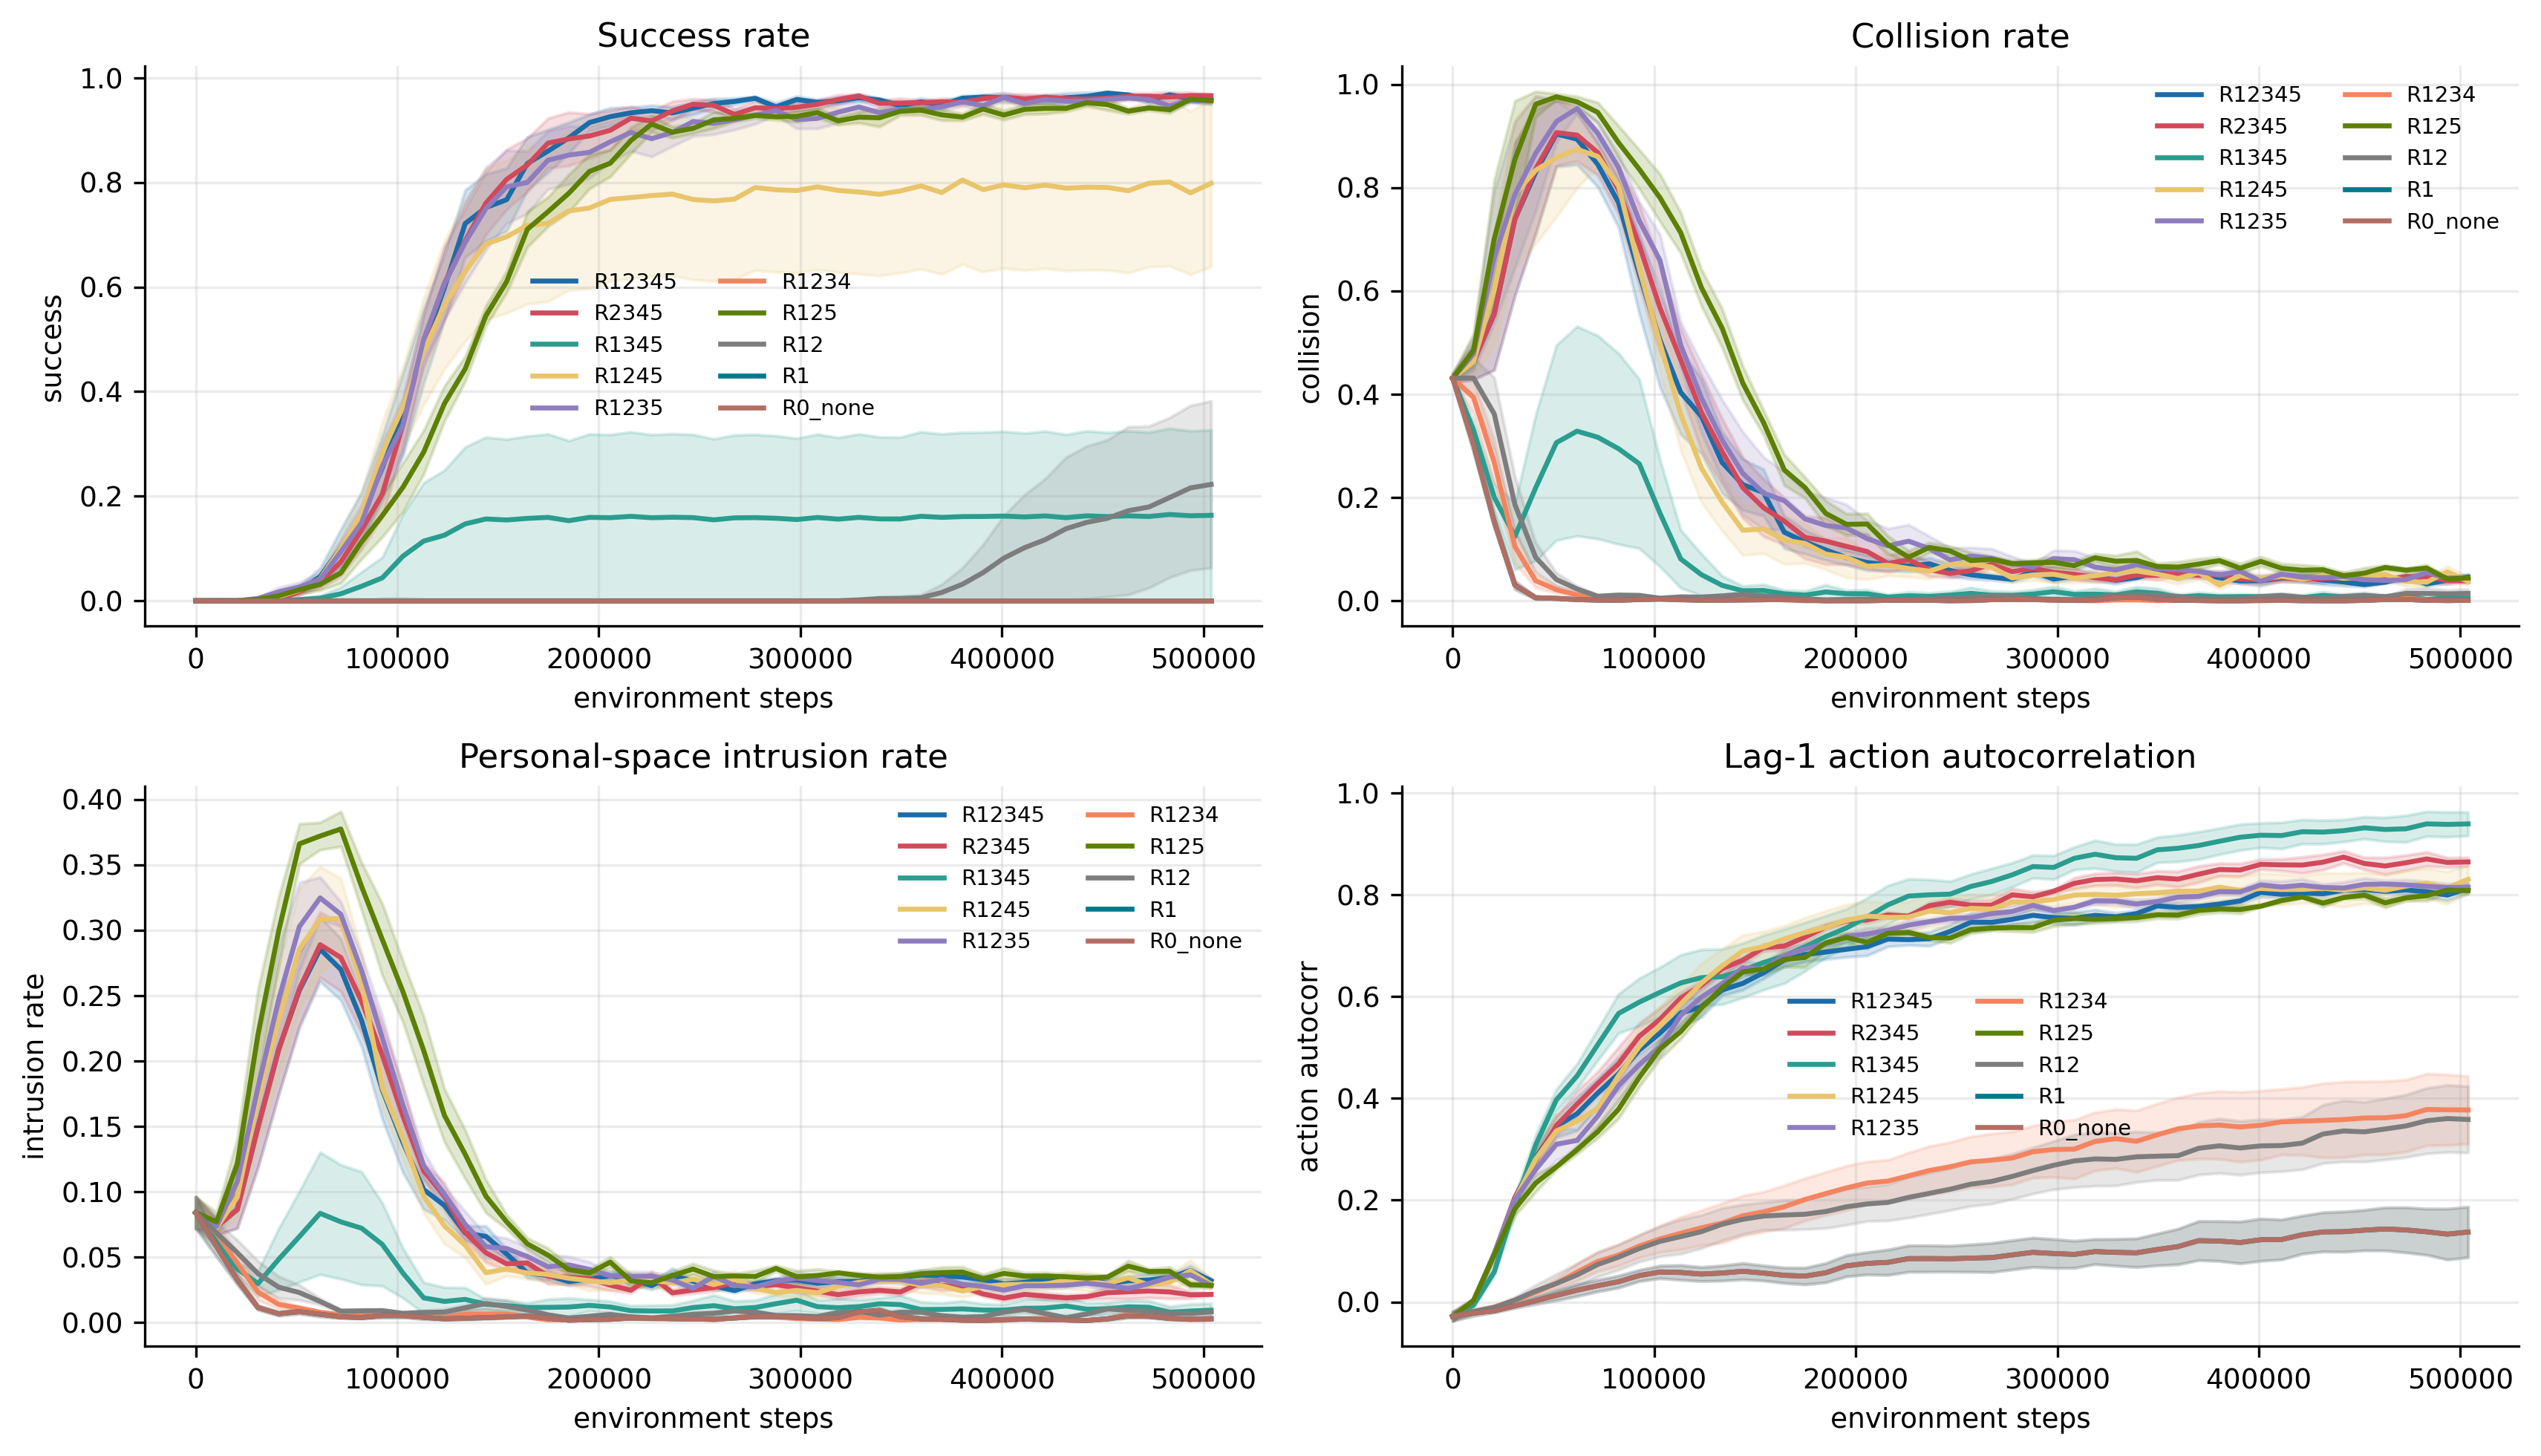
\includegraphics[width=0.84\columnwidth]{fig1_learning_curves.png}
\caption{Training curves, mean $\pm$ s.e.m.\ across six seeds, for the
leave-one-out family and selected sparse arms. The full reward converges by about
$250$k steps, while $R_{1234}$ (no jerk) and the task-only arm never leave zero.
The collision panel shows the characteristic transient in which a policy first
learns to move---and therefore to collide---before it learns to avoid.}
\label{fig:curves}
\end{figure}

\subsection{The lattice: which terms, not how many}
Table~\ref{tab:bysize} summarises all $32$ cells by the number of active
components. Performance is emphatically \emph{not} a function of how many terms
are on: at two active components the range is $[0.000,0.967]$ and at three
$[0.000,0.975]$, spreads far larger than any difference between groups. Two
regimes appear---every arm containing both $R_2$ and $R_5$ exceeds $0.96$, every
arm lacking $R_5$ caps at $0.281$, and arms with $R_5$ but not $R_2$ cluster near
$0.49$.

\begin{table}[!t]
\centering
\caption{The $2^5$ lattice grouped by number of active components. Spread within
a group dwarfs the difference between groups, and reliability (arms solving all
six seeds) does not increase monotonically with component count either.}
\label{tab:bysize}
\small
\setlength{\tabcolsep}{4pt}
\begin{tabular}{ccccccl}
\toprule
$|S|$ & Arms & Min & Max & 6/6 & 0/6 & Best configuration \\
\midrule
0 & 1  & 0.000 & 0.000 & 0 & 1 & task reward only \\
1 & 5  & 0.000 & 0.486 & 0 & 3 & $R_5$ \\
2 & 10 & 0.000 & 0.967 & 1 & 4 & $R_2R_5$ \\
3 & 10 & 0.000 & 0.975 & 2 & 3 & $R_2R_3R_5$ \\
4 & 5  & 0.000 & 0.978 & 2 & 1 & $R_1R_2R_3R_5$ \\
5 & 1  & 0.983 & 0.983 & 1 & 0 & full reward \\
\bottomrule
\end{tabular}
\end{table}

\subsection{Reliability is a second, dissociated axis}
\label{sec:reliability}
Fourteen of the $32$ arms are \emph{bimodal}: their seeds split between
near-ceiling and complete failure, so the pooled mean describes no individual run.
The four arms containing $R_5$ but not $R_2$ all report means near $0.49$, and in
every case that is three seeds near $0.97$ and three at exactly $0.000$.
Reporting $0.49$ for such an arm is not merely imprecise---it names an outcome
that never occurred.

Separating the two axes gives the cleanest single statement in the study. Ranking
the $32$ arms by seeds solved: \emph{no configuration lacking $R_5$ solves more
than two of six, and none containing $R_5$ solves fewer than one}; six
configurations, all with both $R_2$ and $R_5$, solve all six. Mean success and
reliability are therefore not interchangeable, and an ablation table reporting
only the former cannot distinguish a reward that works from one that works half
the time.

\subsection{Attribution, and how far leave-one-out is from it}
Table~\ref{tab:attribution} and Fig.~\ref{fig:attribution} give the central
result. The Shapley values sum to $0.983$, exactly $v(N)-v(\varnothing)$---a
property of the estimator, not a fit, so the five credits can be read as shares.

\begin{table}[!t]
\centering
\caption{Exact component attribution on success rate over the complete $2^5$
lattice, six seeds. Brackets are percentile bootstrap 95\% intervals over seeds.
TOST tests practical equivalence to the full reward within $\pm0.02$ success.}
\label{tab:attribution}
\small
\setlength{\tabcolsep}{3pt}
\begin{tabular}{llccccc}
\toprule
& Component & Shapley $\phi_i$ & \% & LOO & AOI & TOST \\
\midrule
$R_1$ & goal          & $+0.007$\,\tiny{[.002,.013]}   & 0.7    & $+0.008$ & $0.000$ & \textbf{equiv.}\\
$R_2$ & distance      & $+0.400$\,\tiny{[.209,.572]}   & 40.7   & $+0.818$ & $0.248$ & ---\\
$R_3$ & pers.\ space  & $-0.001$\,\tiny{[-.079,.104]}  & $-0.1$ & $+0.172$ & $0.000$ & ---\\
$R_4$ & time-to-coll. & $-0.066$\,\tiny{[-.151,-.006]} & $-6.7$ & $+0.004$ & $0.000$ & \textbf{equiv.}\\
$R_5$ & jerk          & $+0.643$\,\tiny{[.463,.837]}   & 65.4   & $+0.983$ & $0.486$ & ---\\
\midrule
& \textbf{Sum} & $\mathbf{+0.983}$ & 100.0 & & & \\
\bottomrule
\end{tabular}
\end{table}

\begin{figure*}[!t]
\centering
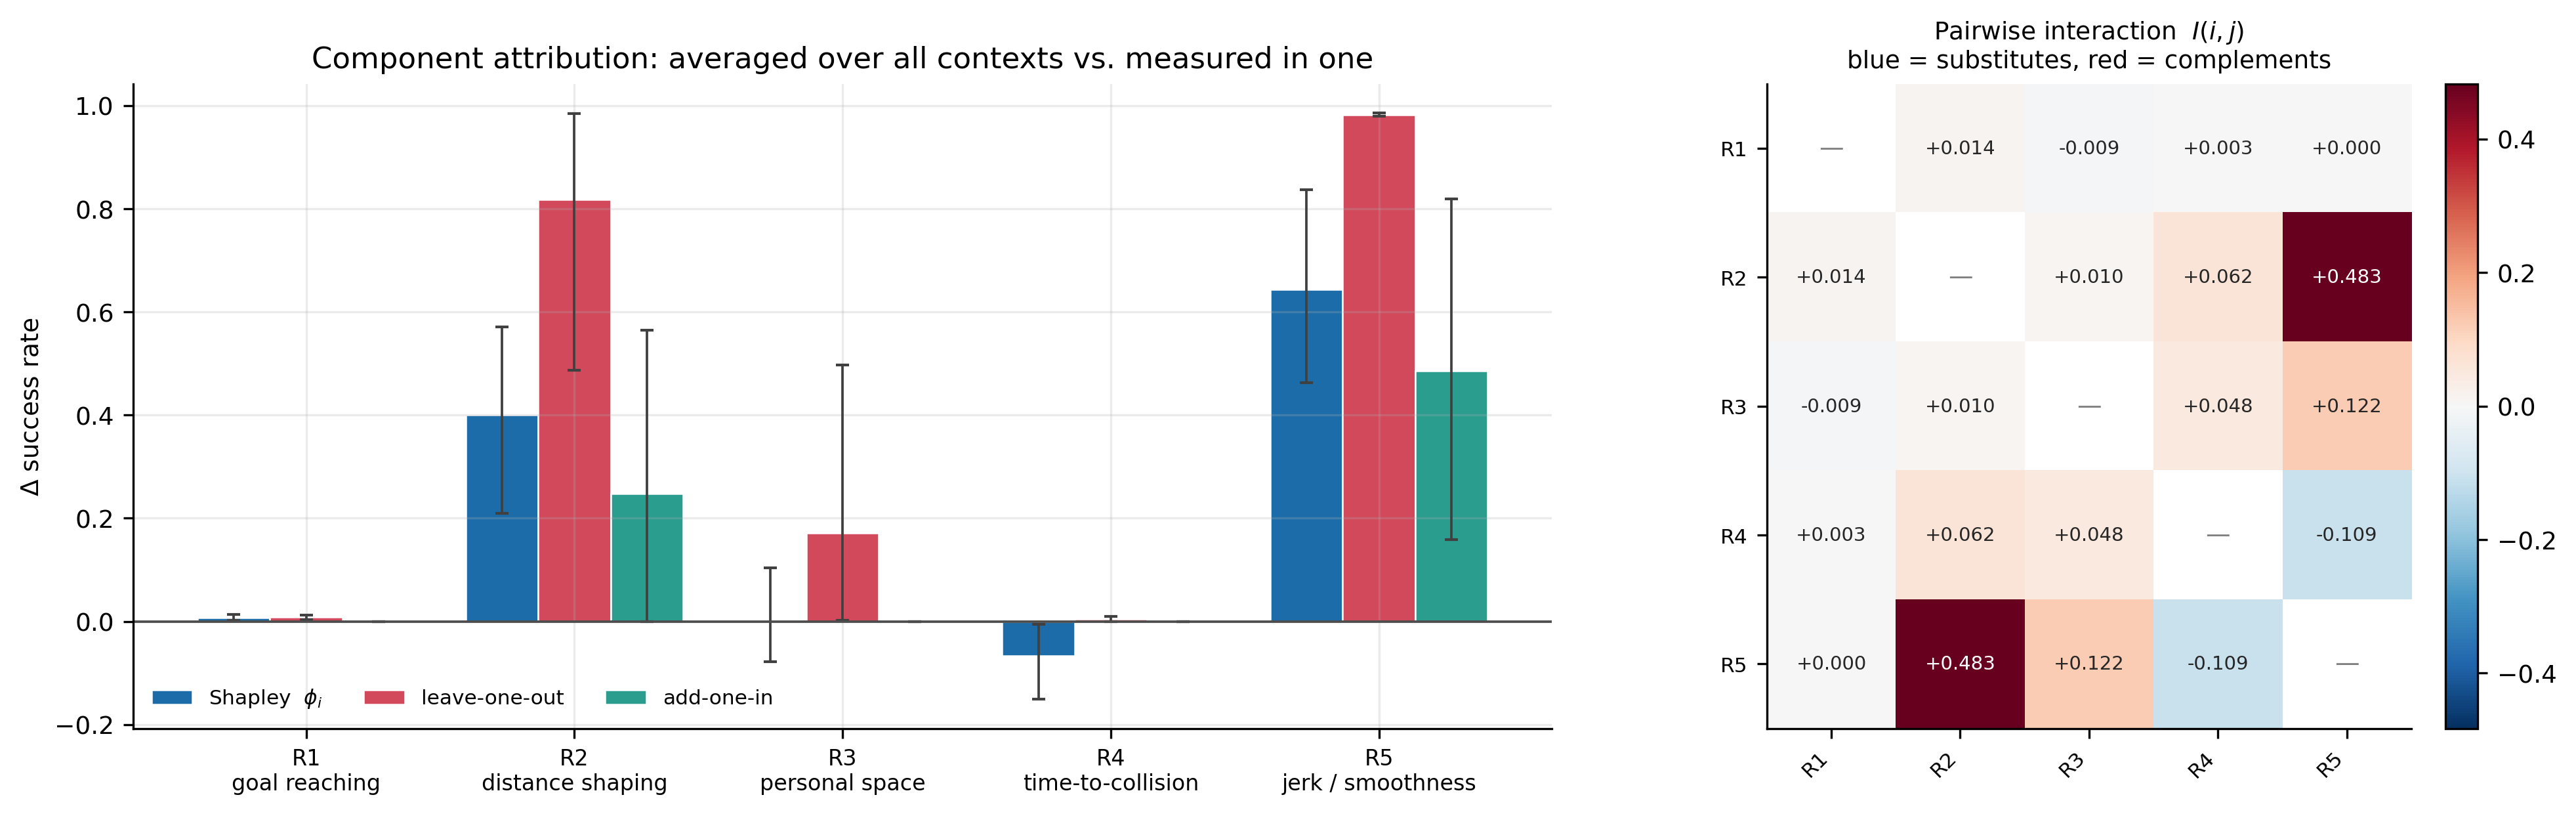
\includegraphics[width=\textwidth]{fig3_attribution_and_interactions.png}
\caption{\textbf{Left:} Shapley value against leave-one-out and add-one-in for
each component, with bootstrap 95\% intervals over six seeds. The disagreement
between the bars is the point---where they diverge, the conventional
single-context ablation reports a property of its context rather than of the
component. \textbf{Right:} pairwise Shapley interaction indices; blue denotes
substitutes, red complements.}
\label{fig:attribution}
\end{figure*}

Two components carry the result. The jerk penalty $R_5$---weighted $0.02$ and
introduced in the literature as a comfort term---accounts for $65.4\%$ of the
total effect ($\phi=+0.643$, $p=0.031$), and distance shaping $R_2$ for $40.7\%$
($\phi=+0.400$, interval excluding zero). The goal bonus $R_1$ contributes
$+0.007$: measurable but negligible, because with a per-step time cost the
fastest way to stop losing reward is already to reach the goal. The
time-to-collision term $R_4$ is mildly \emph{harmful} to success
($\phi=-0.066$), and the personal-space term $R_3$ is indistinguishable from zero.

The gap between the Shapley and LOO columns is the methodological claim made
concrete. For $R_2$, LOO reports $+0.818$ against $\phi=+0.400$, overstating the
contribution by $0.42$ success---a factor of two. For $R_5$ it reports $+0.983$
against $\phi=+0.643$, still dominant but overstated by $0.34$. The clearest case
is $R_3$: LOO $+0.172$ against $\phi=-0.001$, so a single-context ablation credits
the personal-space term with a sixth of the task for a component whose average
contribution is zero. The six seeds show why---the no-$R_3$ arm returns
$\{0.974,\,0.000,\,0.970,\,0.988,\,0.960,\,0.974\}$, and LOO reads that lone
training failure as a component effect. This is exactly the failure mode
Section~\ref{sec:reliability} anticipates: an unreported reliability problem
masquerading as an effect size.

Equivalence testing lets us make positive claims rather than merely failing to
reject: dropping $R_1$ ($p=0.0028$) or $R_4$ ($p=0.0017$) is statistically
equivalent to the full reward within $\pm0.02$ success. For $R_3$ the $90\%$
interval is $[-0.498,+0.154]$ and equivalence is \emph{not} established---this
design lacks the power to resolve $R_3$, which is different from $R_3$ being
inert.

\subsection{Interaction structure explains the bias}
The right panel of Fig.~\ref{fig:attribution} accounts for the divergence. $R_2$
and $R_5$ are strong \textbf{complements}, $I=+0.483$ $[0.205,0.760]$: distance
shaping alone reaches $0.248$ and the jerk penalty alone $0.486$, but together
they reach $0.967$. Neither pays off without the other, so they cannot be tuned
independently, and each one's LOO value is inflated by the other's
presence---exactly the bias measured above. $R_4$ and $R_5$ are
\textbf{substitutes}, $I=-0.109$ $[-0.205,-0.031]$: both suppress high-frequency
velocity change near pedestrians, so with $R_5$ present the anticipatory term is
redundant and its LOO value collapses to $+0.004$. $R_1$ and $R_3$ show a small
but reliable substitution, $I=-0.009$ $[-0.020,-0.003]$. The largest third-order
dividend, $m(\{R_2,R_3,R_5\})=+0.240$, indicates that proxemic shaping becomes
useful only once the policy is already goal-directed and temporally regularised.
Per Section~\ref{sec:stats}, these classifications rest on the bootstrap
intervals; the Holm-adjusted $p$ for ten pairs cannot fall below $0.31$ at six
seeds under any effect size.

\subsection{One metric is not enough}
Table~\ref{tab:multimetric} gives the Shapley value of every component on six
metrics, and it changes several conclusions drawn from success alone.

\begin{table}[!t]
\centering
\caption{Shapley value of each component across six evaluation metrics, computed
independently on the same lattice. Arrows mark the desirable direction. $R_4$ is
the only component that improves both proxemic metrics.}
\label{tab:multimetric}
\small
\setlength{\tabcolsep}{2.6pt}
\begin{tabular}{lcccccc}
\toprule
& Success & Collision & Min.\ sep. & Intrusions & Nav.\ time & Accel. \\
& $\uparrow$ & $\downarrow$ & [m] $\uparrow$ & $\downarrow$ & [s] $\downarrow$ & $\downarrow$ \\
\midrule
$R_1$ & $+0.007$ & $-0.004$ & $-0.026$ & $+0.095$ & $-0.80$ & $+0.005$ \\
$R_2$ & $+0.400$ & $+0.014$ & $-0.440$ & $+0.337$ & $-4.12$ & $+0.413$ \\
$R_3$ & $-0.001$ & $-0.004$ & $+0.009$ & $-0.072$ & $-0.07$ & $-0.022$ \\
$R_4$ & $-0.066$ & $-0.003$ & $\mathbf{+0.079}$ & $\mathbf{-0.090}$ & $+0.77$ & $-0.044$ \\
$R_5$ & $+0.643$ & $+0.018$ & $-0.621$ & $+0.664$ & $-7.01$ & $\mathbf{-0.376}$ \\
\bottomrule
\end{tabular}
\end{table}

Three readings follow. (i) $R_4$, which \emph{costs} $0.066$ success, is the only
component improving both proxemic metrics, buying $+0.079$\,m of minimum
separation $[0.024,0.149]$ and $0.090$ fewer intrusions $[-0.166,-0.019]$ for
$0.77$\,s of navigation time---a defensible trade for a socially aware navigator,
and invisible in a success-only table. (ii) The large negative separation values
for $R_2$ and $R_5$ are a compositional artefact, not antisocial behaviour: arms
lacking them time out without moving, and a robot that never leaves its start
position trivially maintains separation and records no intrusions. Proxemic
metrics must therefore be read jointly with success, never instead of it.
(iii) $R_5$ does reduce mean squared acceleration ($\phi=-0.376$), performing its
nominal comfort function---but that is not where its value comes from.

\subsection{Why a $0.02$-weighted smoothness term dominates}
\label{sec:jerk}
That a comfort term should carry two thirds of the result demands an explanation.
We argue $R_5$ is not functioning as a comfort preference at all, but as an
implicit \emph{exploration-annealing} term.

During training, actions are sampled as $a_t\sim\mathcal{N}(\mu_t,\sigma^2I)$
with state-independent $\sigma$. Taking the expectation of the jerk penalty under
independent sampling,
\begin{equation}
\mathbb{E}\big[-w_j\lVert a_t-a_{t-1}\rVert^2\big]
=-w_j\lVert\mu_t-\mu_{t-1}\rVert^2-4w_j\sigma^2,
\label{eq:variance}
\end{equation}
so $R_5$ places a direct quadratic penalty on the policy's exploration variance.
With $\texttt{ent\_coef}=0$ nothing opposes it, and it therefore acts as a learned
annealing schedule on $\sigma$---the mirror image of the entropy bonus used to
\emph{sustain} exploration in maximum-entropy methods \cite{haarnoja2018soft}.
Two predictions follow, and both hold.

\emph{(i) Final policy variance should separate on the presence of $R_5$.} It
does, perfectly. Across all $32$ arms, every configuration containing $R_5$ ends
training with $\sigma\in[0.302,0.333]$ (mean $0.316\pm0.018$) and every
configuration lacking it with $\sigma\in[0.406,0.463]$ (mean $0.433\pm0.036$),
from a common initialisation of $0.607$. The two sets do not overlap, and
$\sigma_{\text{end}}$ correlates with success at $r=-0.69$ across arms. The three
collapsed runs noted in Section~IV all sit in the high-$\sigma$ group.

\emph{(ii) The weight response should be non-monotone.} A comfort-preference
account predicts that more smoothness can only make the agent's own reward easier
to collect, so success should rise and saturate. An annealing account predicts an
optimum: too little and $\sigma$ stays high so the goal is never reached; too
much and $\sigma$ collapses before a competent policy is found.
Fig.~\ref{fig:jerk} shows a sharp threshold and then decline---$0.000$ for
$w_j\le0.005$, $0.329$ at $0.01$, $0.965$ at $0.02$, $0.873$ at $0.05$, then
$0.508$ at $0.10$, with the collision rate rising to $0.496$ as the policy
converges prematurely.

\begin{figure}[!t]
\centering
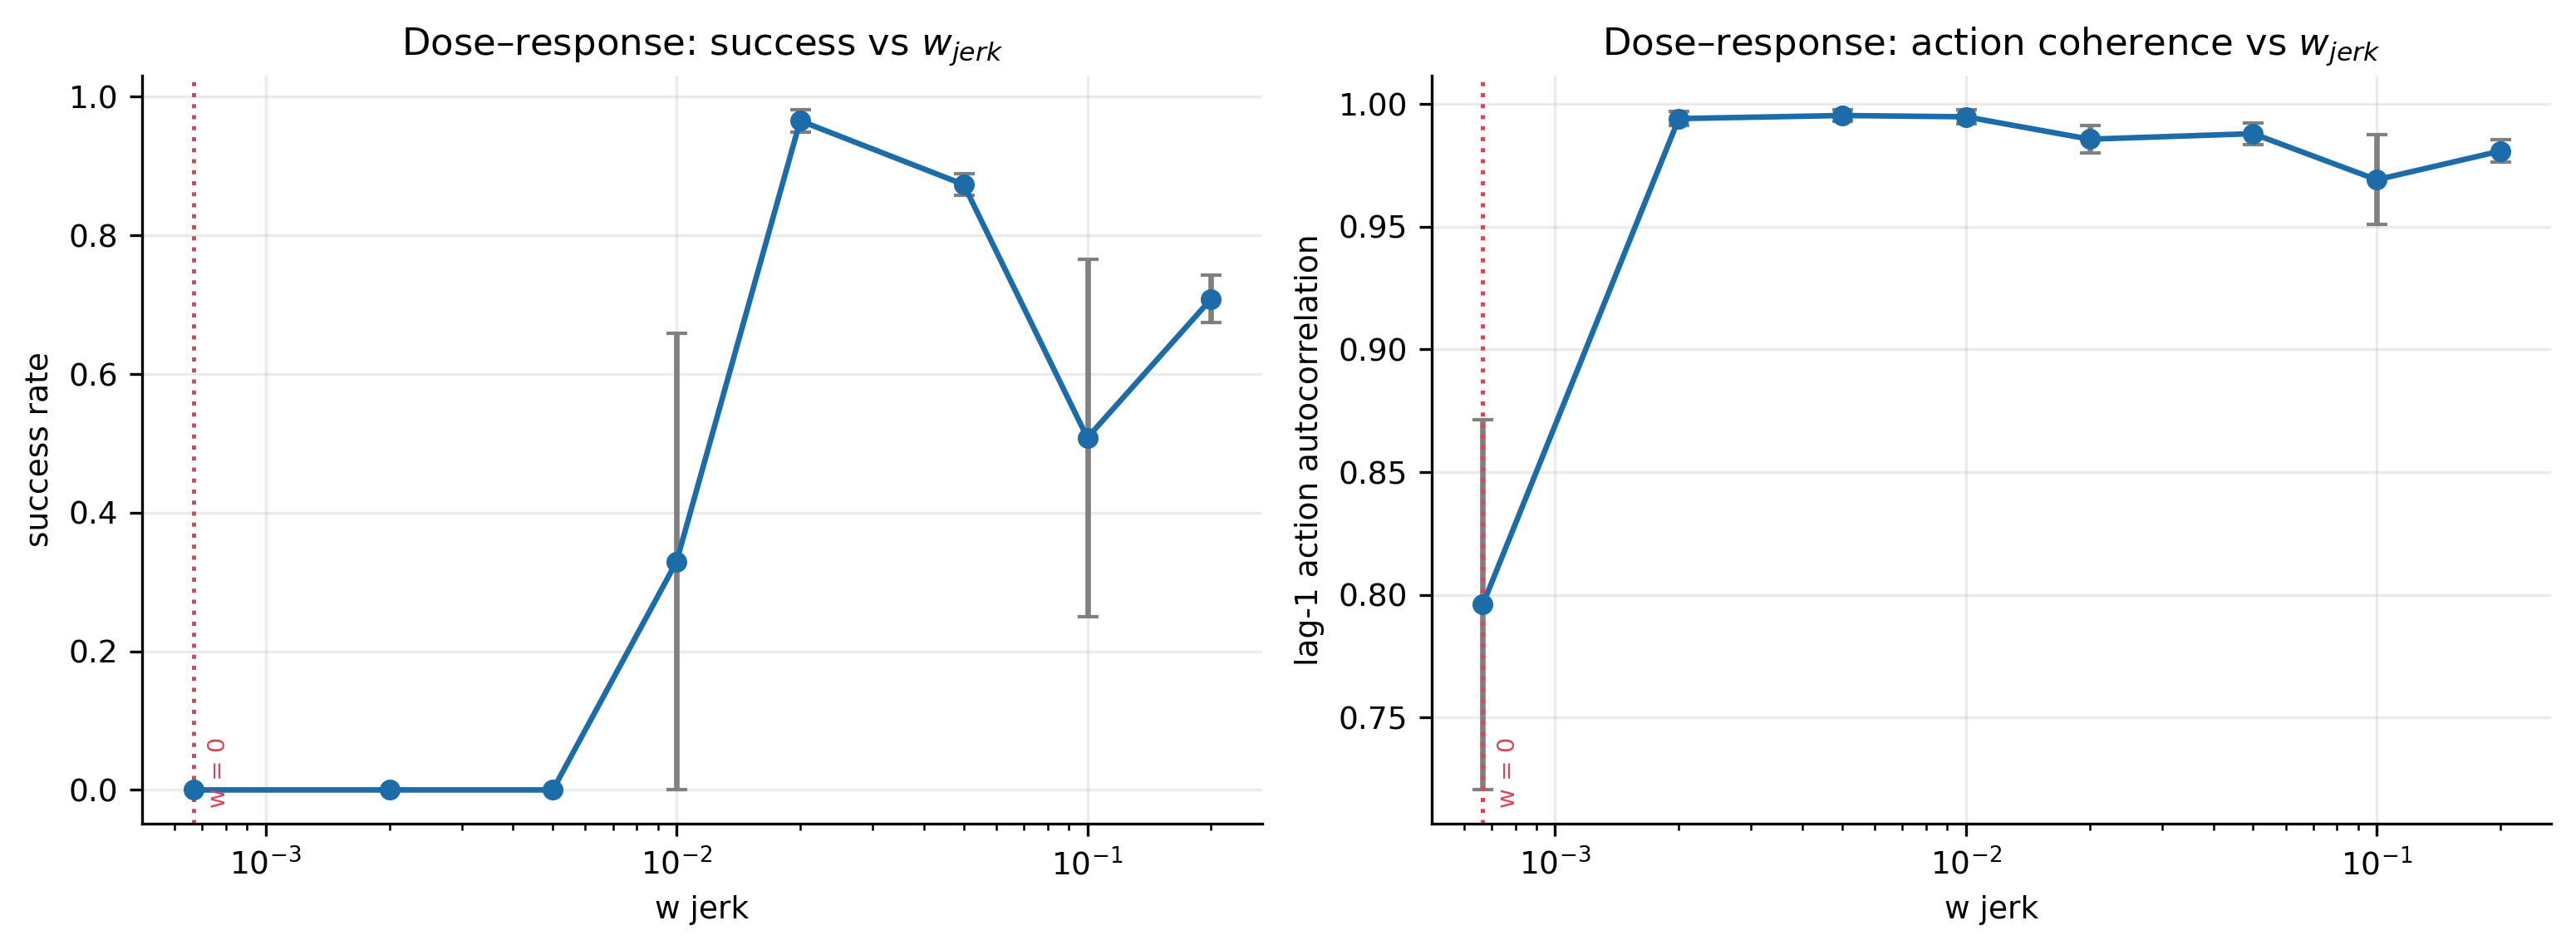
\includegraphics[width=0.92\columnwidth]{fig8_jerk_mechanism.png}
\caption{Weight sweep for $R_5$ over two orders of magnitude (3 seeds, $250$k
steps). \textbf{Left:} success is sharply non-monotone with an optimum near
$w_j=0.02$, which a comfort-preference account cannot produce. \textbf{Right:}
lag-1 action autocorrelation has already saturated at $w_j=0.002$, where success
is still zero---so smoothness of the executed trajectory is not the operative
variable.}
\label{fig:jerk}
\end{figure}

One control rules out the simpler explanation. We also measured lag-1 action
autocorrelation at evaluation (Fig.~\ref{fig:jerk}, right). It is \emph{not} the
discriminating variable: at $w_j=0.002$ the deterministic policy is already highly
autocorrelated ($0.994$) yet achieves $0.000$ success, while the optimum at
$w_j=0.02$ has slightly \emph{lower} autocorrelation ($0.986$) and $0.965$
success. Temporal smoothness of the executed trajectory is therefore not what
$R_5$ buys; the variance of the training-time action distribution is.

\subsection{Shaping form: invariance is neither costly nor useful here}
\label{sec:form}
Holding the component set fixed and replacing the potential-based form of $R_2$
with the naive per-step progress reward changes success by $-0.006$ with all five
components present ($0.976$ versus $0.983$) and by $+0.007$ with the goal bonus
removed ($0.981$ versus $0.975$); neither exceeds the seed-to-seed spread, and
navigation time and path-length ratio are likewise within noise. The
policy-invariance guarantee of \cite{ng1999policy} therefore costs nothing here
but buys nothing measurable either---a useful negative result, since the invariant
form is the more troublesome to implement correctly.

%=============================================================================
\section{Discussion and Limitations}
%=============================================================================
The practical recommendation from Table~\ref{tab:attribution} is not ``use all
five terms.'' It is: a temporal-regularisation term and a dense distance term are
jointly load-bearing and must be tuned together; a sparse goal bonus is redundant
once a per-step time cost is present; and the social terms should be justified on
proxemic metrics, where they pay, not on success rate, where they do not.

More broadly, the $R_5$ result is a warning about reading reward ablations at face
value. A term introduced for one reason (comfort) can dominate for an entirely
different one (exploration control), and a single-context ablation cannot tell the
two apart. Where a shaping term acts on the optimiser rather than the task, its
``importance'' is a statement about the training algorithm as much as the
objective \cite{andrychowicz2021what}---so it need not transfer to a different
algorithm, a question worth asking of any published reward ablation.

\textbf{Limitations.} (i) Simulation only, with perfect state observation and no
occlusion; sim-to-real transfer is not demonstrated. (ii) ORCA pedestrians are
reciprocal and deterministic and lack intent, groups and social convention, so our
conclusions concern proxemic geometry rather than human comfort; the stronger
claim requires a user study. (iii) Weights are fixed and only switched on or off,
so a component could underperform through mis-scaling; the dose--response sweep
addresses this for $R_5$, and the interaction table identifies which pairs must
be swept jointly. (iv) One scenario family at one
pedestrian density; terms that are substitutes here need not be in a corridor.
(v) Equal budget is itself a choice---two seeds of $R_1R_2$ begin to learn only
after $400$k steps (Fig.~\ref{fig:curves}), so that arm's $0.281$ is a statement
about $500$k steps, not about the reward. (vi) Six seeds is the minimum for which
an exact two-sided permutation test can reach $p<0.05$, which is why $R_3$ remains
unresolved rather than confirmed inert. (vii) The mechanism argument of
Section~\ref{sec:jerk} rests on Eq.~\eqref{eq:variance}, the $\sigma$ separation and the non-monotone dose
response; a direct intervention---supplying temporal coherence from the dynamics
through an action low-pass filter while holding $w_j=0$---would close it, and is
our immediate next step. (viii) Shaping is not the only route to safety:
control-barrier-function filters enforce it structurally \cite{ames2016control},
and benchmarking a shaped-reward policy against a filtered one would separate
what the reward must supply from what a controller can guarantee.

%=============================================================================
\section{Conclusion}
%=============================================================================
We ran the complete $2^5$ factorial over five reward-shaping components for
socially aware robot navigation and computed exact Shapley attribution from it.
Leave-one-out ablation, the field's default instrument, overstates one component's
contribution twofold and assigns $+0.172$ success to a component whose true
contribution is zero; the interaction decomposition shows why, identifying one
complementary pair and two substitute pairs. The dominant component is a nominally
minor jerk penalty operating as an implicit exploration-annealing term rather than
a comfort preference, with final policy variance separating perfectly on its
presence and the same separation governing reliability. The full reward reaches
$0.983$ success against $0.714$ for a tuned ORCA planner. We recommend that reward
ablations report attribution over a factorial design and reliability alongside
mean performance, or state explicitly that their single-context numbers are
conditional on the presence of every other term.

%=============================================================================
%  References
%=============================================================================
\balance
\begin{thebibliography}{99}

\bibitem{mavrogiannis2023core}
C.~Mavrogiannis \emph{et al.}, ``Core challenges of social robot navigation: A
survey,'' \emph{ACM Trans. Human-Robot Interact.}, vol.~12, no.~3,
pp. 1--39, 2023.

\bibitem{chen2019crowdrobot}
C.~Chen, Y.~Liu, S.~Kreiss, and A.~Alahi, ``Crowd-robot interaction: Crowd-aware
robot navigation with attention-based deep reinforcement learning,'' in
\emph{Proc. IEEE Int. Conf. Robot. Autom. (ICRA)}, 2019, pp.
6015--6022.

\bibitem{chen2017socially}
Y.~F. Chen, M.~Everett, M.~Liu, and J.~P. How, ``Socially aware motion planning
with deep reinforcement learning,'' in \emph{Proc. IEEE/RSJ Int. Conf. Intell. Robots Syst. (IROS)}, 2017, pp. 1343--1350.

\bibitem{liu2021decentralized}
S.~Liu, P.~Chang, W.~Liang, N.~Chakraborty, and K.~Driggs-Campbell,
``Decentralized structural-RNN for robot crowd navigation with deep reinforcement
learning,'' in \emph{Proc. IEEE Int. Conf. Robot. Autom. (ICRA)}, 2021,
pp. 3517--3524.

\bibitem{shapley1953value}
L.~S. Shapley, ``A value for $n$-person games,'' in \emph{Contributions to the
Theory of Games II}, H.~W. Kuhn and A.~W. Tucker, Eds. Princeton, NJ: Princeton
Univ. Press, 1953, pp. 307--317.

\bibitem{harsanyi1963simplified}
J.~C. Harsanyi, ``A simplified bargaining model for the $n$-person cooperative
game,'' \emph{Int. Econ. Rev.}, vol.~4, no.~2, pp. 194--220, 1963.

\bibitem{grabisch1999axiomatic}
M.~Grabisch and M.~Roubens, ``An axiomatic approach to the concept of interaction
among players in cooperative games,'' \emph{Int. J. Game Theory}, vol.~28, no.~4, pp. 547--565, 1999.

\bibitem{vandenberg2011reciprocal}
J.~van~den Berg, S.~J. Guy, M.~Lin, and D.~Manocha, ``Reciprocal $n$-body
collision avoidance,'' in \emph{Robotics Research (ISRR)}, Springer Tracts in Advanced Robotics, vol.~70, 2011, pp. 3--19.

\bibitem{trautman2010unfreezing}
P.~Trautman and A.~Krause, ``Unfreezing the robot: Navigation in dense,
interacting crowds,'' in \emph{Proc. IEEE/RSJ Int. Conf. Intell. Robots Syst. (IROS)}, 2010, pp. 797--803.

\bibitem{chen2017decentralized}
Y.~F. Chen, M.~Liu, M.~Everett, and J.~P. How, ``Decentralized non-communicating
multiagent collision avoidance with deep reinforcement learning,'' in \emph{Proc.
IEEE Int. Conf. Robotics and Automation (ICRA)}, 2017, pp. 285--292.

\bibitem{hall1966hidden}
E.~T. Hall, \emph{The Hidden Dimension}. New York, NY: Doubleday, 1966.

\bibitem{alyassi2025social}
R.~Alyassi, C.~Cadena, R.~Riener, and D.~Paez-Granados, ``Social robot
navigation: A review and benchmarking of learning-based methods,''
\emph{Front. Robot. AI}, vol.~12, art.~1658643, 2025.

\bibitem{ng1999policy}
A.~Y. Ng, D.~Harada, and S.~Russell, ``Policy invariance under reward
transformations: Theory and application to reward shaping,'' in \emph{Proc. 16th Int. Conf. Mach. Learn. (ICML)}, 1999, pp. 278--287.

\bibitem{lundberg2017unified}
S.~M. Lundberg and S.-I. Lee, ``A unified approach to interpreting model
predictions,'' in \emph{Adv. Neural Inf. Process. Syst. (NeurIPS)}, vol.~30, 2017, pp. 4765--4774.

\bibitem{henderson2018deep}
P.~Henderson, R.~Islam, P.~Bachman, J.~Pineau, D.~Precup, and D.~Meger, ``Deep
reinforcement learning that matters,'' in \emph{Proc. 32nd AAAI Conf. Artif. Intell.}, 2018, pp. 3207--3214.

\bibitem{agarwal2021precipice}
R.~Agarwal, M.~Schwarzer, P.~S. Castro, A.~Courville, and M.~G. Bellemare,
``Deep reinforcement learning at the edge of the statistical precipice,'' in
\emph{Adv. Neural Inf. Process. Syst. (NeurIPS)}, vol.~34,
2021, pp. 29304--29320.

\bibitem{andrychowicz2021what}
M.~Andrychowicz \emph{et al.}, ``What matters for on-policy deep actor-critic
methods? A large-scale study,'' in \emph{Int. Conf. Learn. Represent. (ICLR)}, 2021.

\bibitem{lakens2017equivalence}
D.~Lakens, ``Equivalence tests: A practical primer for $t$ tests, correlations,
and meta-analyses,'' \emph{Soc. Psychol. Personal. Sci.},
vol.~8, no.~4, pp. 355--362, 2017.

\bibitem{schulman2017proximal}
J.~Schulman, F.~Wolski, P.~Dhariwal, A.~Radford, and O.~Klimov, ``Proximal
policy optimization algorithms,'' \emph{arXiv preprint arXiv:1707.06347}, 2017.

\bibitem{raffin2021sb3}
A.~Raffin, A.~Hill, A.~Gleave, A.~Kanervisto, M.~Ernestus, and N.~Dormann,
``Stable-Baselines3: Reliable reinforcement learning implementations,''
\emph{J. Mach. Learn. Res.}, vol.~22, no.~268, pp. 1--8, 2021.

\bibitem{haarnoja2018soft}
T.~Haarnoja, A.~Zhou, P.~Abbeel, and S.~Levine, ``Soft actor-critic: Off-policy
maximum entropy deep reinforcement learning with a stochastic actor,'' in
\emph{Proc. 35th Int. Conf. Mach. Learn. (ICML)}, 2018, pp. 1861--1870.

\bibitem{ames2016control}
A.~D. Ames, X.~Xu, J.~W. Grizzle, and P.~Tabuada, ``Control barrier function
based quadratic programs for safety critical systems,'' \emph{IEEE Trans. Autom. Control}, vol.~62, no.~8, pp. 3861--3876, 2017.

\end{thebibliography}

\end{document}
